\title{\Large \textbf{Modelling the Age of Abalone}}
\author{\small 450132759}
\date{\small October 29, 2018}

\documentclass[9pt,twocolumn]{article}
%\usepackage{fullpage} % full parge margins
\usepackage[margin=0.5in]{geometry}
\usepackage{hyperref} % allows for linking urls
\usepackage[superscript,biblabel]{cite} % superscript while citing
\usepackage{booktabs}
\usepackage{graphicx} % allows for adding figures
\usepackage{subcaption} % allows for adding subfigures
\usepackage{enumitem} % allows for lists
\usepackage{amsmath} % allows for math equations
\usepackage{gensymb} % degree symbol, usage: \degree
\usepackage{csvsimple}
\usepackage{booktabs} % to generate booktabs style tables
\usepackage{lscape}
\usepackage{siunitx}
\usepackage{tikz} % To generate the plot from csv
\usepackage{pgfplots}
\pgfplotsset{compat=newest} % Allows to place the legend below plot
\usepackage{placeins} % Use in conjunction with \FloatBarrier to limit floating of figures
\usepackage{sectsty} % allows for defining section styles
\sectionfont{\fontsize{12}{13}\selectfont} % defines font size of sections

\begin{document}
	\begin{center}
		\textbf{\Large Modelling the Age of Abalone} \\\vspace{4mm}
		\texttt{450132759 / 450237777\\470315518 / 470396894}
	\end{center}
	\begin{abstract}
		The Blacklip Abalone, scientific name Haliotis rubra, is common to several parts of Australia \cite{source}. They are fished recreationally and also farmed. A data set provided by University of California Irvine, originally from the Department of Primary Industry and Fisheries, Tasmania, consists of several physical characteristics, including the number of rings of the Blacklip Abalone shell. The number of rings acts as proxy for the age of the Abalone. We set out to determine and compare both the best and most practical model of age of the abalone using multiple regression. This could then be used to develop and enforce recreational fishing regulations and also to maintain helathy farmed populations. Beginning with a full model, we employ step backward model selection using the Akaike information criterion (AIC). This is compared with a step forward AIC and also a practical model using easy to measure explantory variables. The practical model first removes highly correlated variables using a test for multicollinearity. We then remove difficult to measure explantory variables and test the performance of the resultant model. Our analysis finds that a practical model performs well compared to the stepwise model and can form the basis for developing best harvesting practices both recreationally and for the Blacklip Abalone Farming industry.
	\end{abstract}

	\section{Introduction}
		Abalone meat is used as a food delicacy, its shells are a foundation for certain types of jewellery and it functions ecologically to stablize kelp forrests and algae in its rocky reef habitat. Blacklip Abalone reach sexual maturity after three to six years and spawning occurs between Spring and Autumn\cite{blacklip}. Given the importance of a healthy Abalone population, both in the wild and when farmed, it is crucial to develop, apply and regulate best harvesting practices to maintain healthy Abalone populations. With this in mind, we question how well an unrestriced model using all explanatory variables predicts the age of the Blacklip Abalone. An attempt is then made to build a practical model that can be deployed by farmers and regulators allike that provides a similar level of predictive power but doesn't necessitate killing the Abalone or require the use of specialized equipment.					
	\section{Data Set}
	
		The data is provided by the Machine Leanring Repository at University of California Irvine. It was orginally obtained from the Department of Primary Industry and Fisheries, Tasmania. The variables are:
		\begin{table}[!htbp]
			\resizebox{\columnwidth}{!}{%
				\begin{tabular}{@{}llll@{}}
					\toprule
					Variable        & Type       & Dimension & Description                 \\ \midrule
					Sex             & nominal    &           & M, F and I (infant)         \\
					Length          & continuous & mm        & Longest shell measurement   \\
					Diameter        & continuous & mm        & perpendicular to length     \\
					Height          & continuous & mm        & with meat in shell          \\
					Whole\_weight   & continuous & g         & whole abalone               \\
					Shucked\_weight & continuous & g         & weight of meat              \\
					Viscera\_weight & continuous & g         & gut weight (after bleeding) \\
					Shell\_weight   & continuous & g         & after being dried           \\
					Rings           & integer    &           & + 1.5 gives age in years    \\ \bottomrule
				\end{tabular}%
			}
			\caption{Description of Data Set}
		\end{table}	
		
		After assigning new variable names to each column, we checked the assumption for multicollinearity. Linear regression assumes that there is little or no multicollinearity in the data; however, from the ggpairs output, most of the variables were relatively highly correlated with one another. The variables with few of the highest correlations were between length and diameter, as well as whole weight and the other weight predictors. Moreover, we found out that despite the difference in their means, male and female seemed to have similar distributions. So from such results, we decided to combine male and female into one category along with removing either length, or diameter from the model.
		
		\begin{figure}[!htbp]
			\centering
			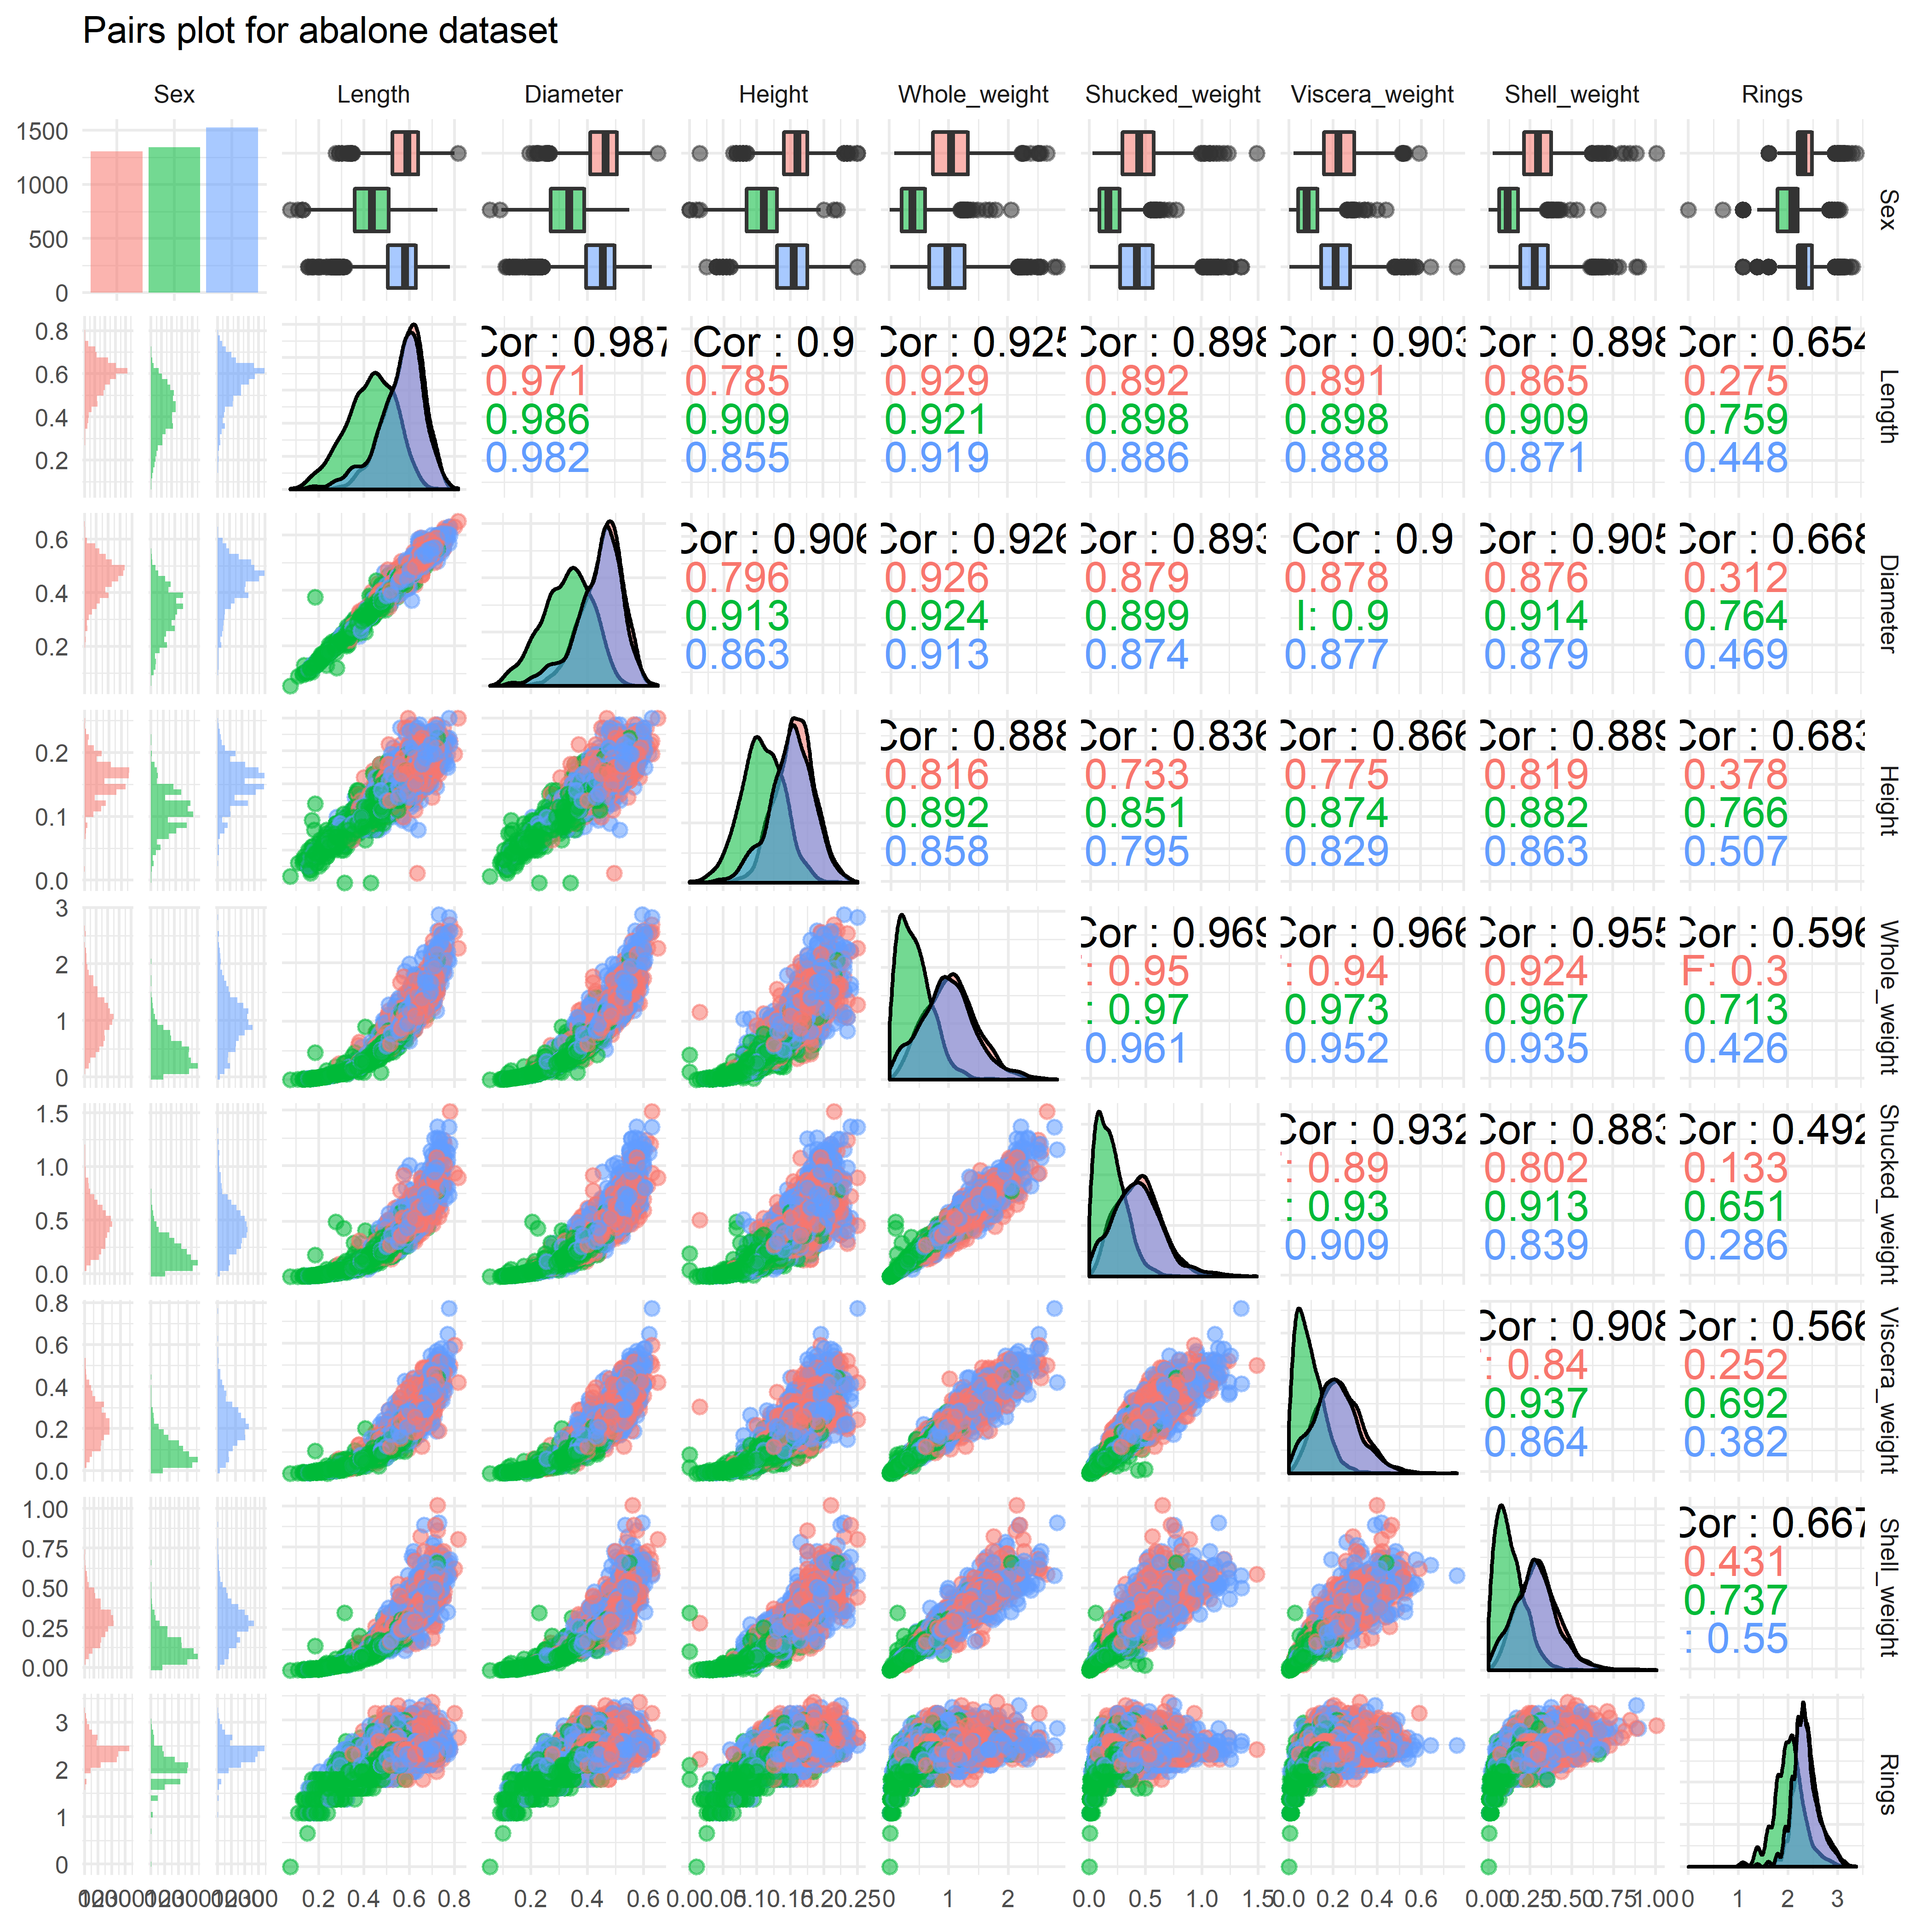
\includegraphics[width=0.85\columnwidth]{ggpairs}
			\caption{}
			\label{fig:ggpairs}
		\end{figure}
		
		
	\section{Analysis}
	
	\begin{figure}[!htbp]
		\centering
		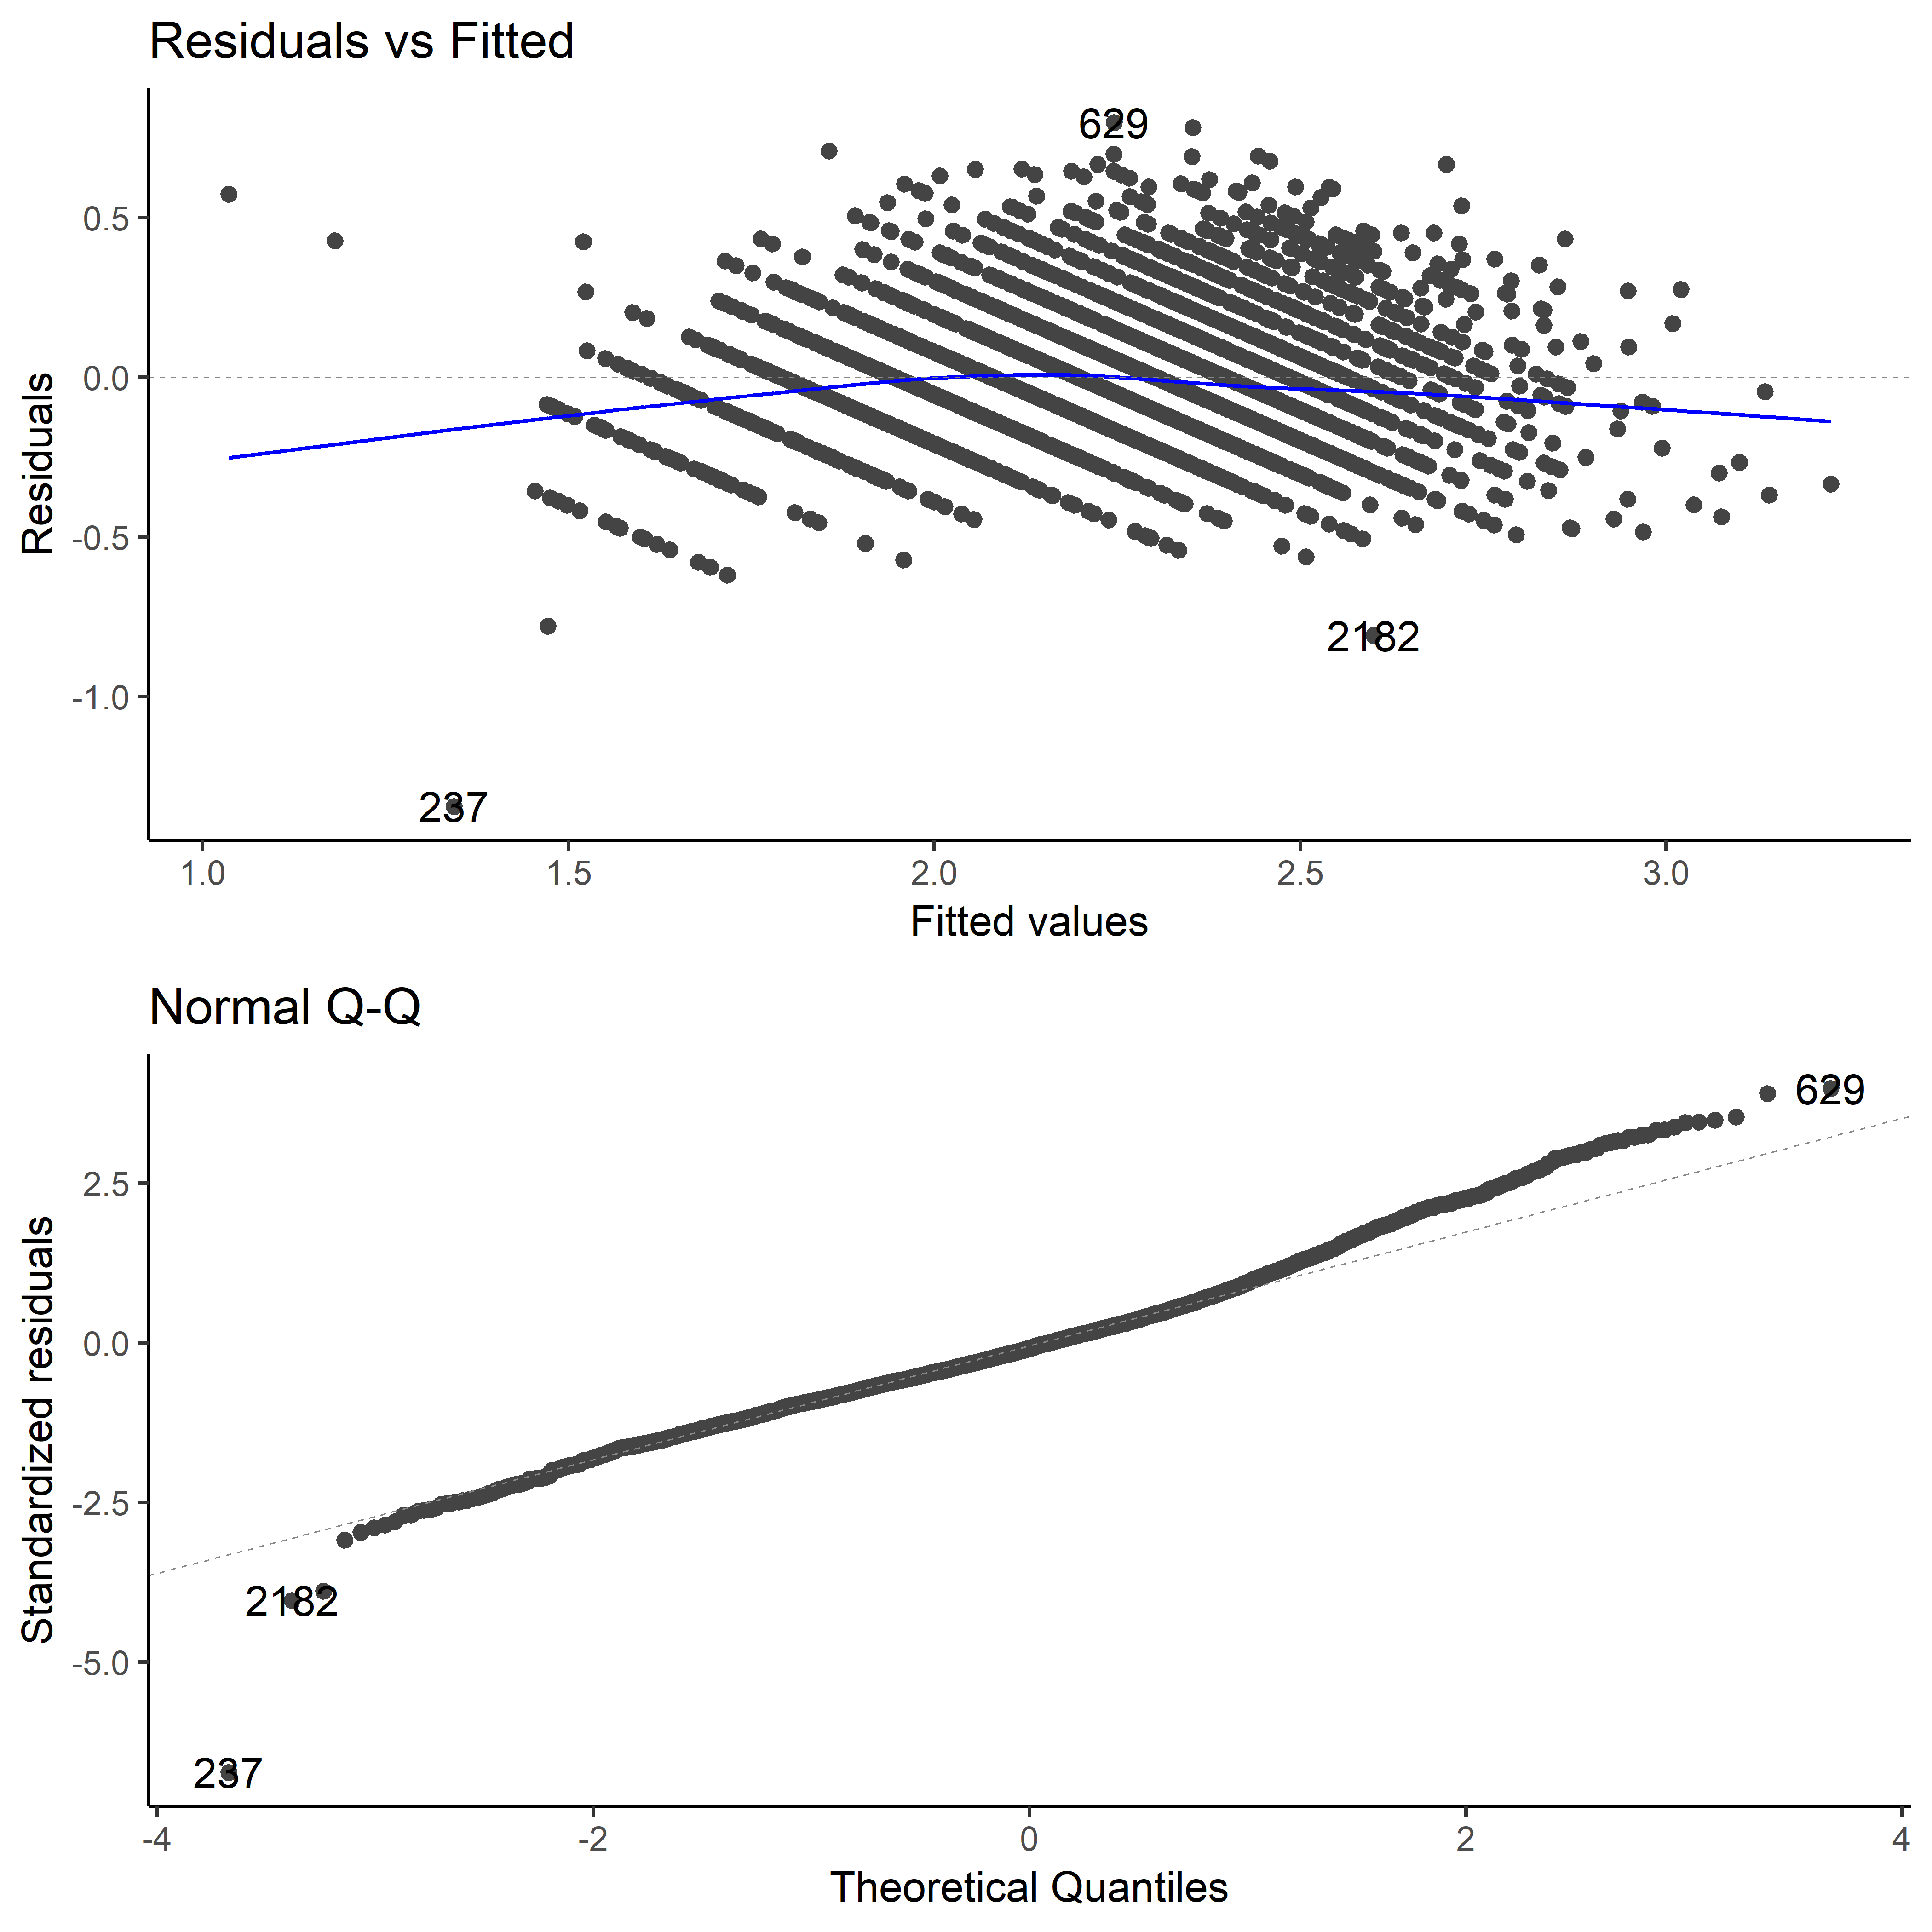
\includegraphics[width=0.7\linewidth]{varnorm}
		\caption{}
		\label{fig:varnorm}
	\end{figure}
	
	
	\section{Results}
	
	\section{Discussion \& Conclusion}
	
	\section{Appendix}
	
	\begin{thebibliography}{9}
		\bibitem{source}
		Abalone. (2018). Dpipwe.tas.gov.au. Retrieved 27 October 2018, from \url{https://dpipwe.tas.gov.au/sea-fishing-aquaculture/community-resources/fish-facts/abalone-blacklip}
		
		\bibitem{blacklip}
		Wild Fisheries Research Program. (2018). Dpi.nsw.gov.au. Retrieved 27 October 2018, from		\url{https://www.dpi.nsw.gov.au/__data/assets/pdf_file/0009/375858/BlacklipAbalone.pdf}
	\end{thebibliography}
\end{document}





























